\documentclass{lintelo/lintelo}
\usepackage{placeins}

\addbibresource{references.bib}

\title{Project Speed Camera}
\author{Thomas in 't Anker, Lars Faase, Niek Kuipers, Max te Lintelo}
\releasedate{\lindate\today}
\documentstatus{Concept}
\documenttype{Research Document}
\documenttypeabbreviation{RD}

\begin{document}

\maketitle

\begin{lindocumenthistory}
    \lindocumenthistoryrow{\TODO{2023-03-03}}{Concept}{Initial version.}
\end{lindocumenthistory}

\begin{lindistributionlist}{R01}
    \lintablerow{Thomas in 't Anker & Author   & x }
    \lintablerow{Lars Faase         & Author   & x }
    \lintablerow{Niek Kuipers       & Author   & x }
    \lintablerow{Max te Lintelo     & Author   & x }
    \lintablerow{Jonathan Overes    & Reviewer &   }
    \lintablerow{Joan Schrasser     & Client   &   }
\end{lindistributionlist}

\begin{linissues}
    \linissue{\TODO{1.}}{\cref{chap:development-board}}{DONE: \st{Complete research for development board.}}{Max te Lintelo}{2023-03-03}
    \linissue{\TODO{2.}}{\cref{chap:camera}}{Add camera research.}{Lars Faase}{2023-03-03}
    \linissue{\TODO{3.}}{\cref{chap:license-plate-recognition}}{Add ALPR research.}{Niek Kuipers}{2023-03-03}
    \linissue{\TODO{4.}}{\cref{chap:speed-detection}}{Add speed detection research.}{Thomas in 't Anker}{2023-03-03}
\end{linissues}

\lintableofcontents
\linlistoffigures
\linlistoftables
%\linlistoflistings

\linreferences

\chapter{\REVIEW{Introduction}}
\label{chap:introduction}

This document is written to provide the research required to build a hidden speed camera.
The question that this research paper will try to answer is: "How can we make a speed camera that logs the speed and number plate of road users?"
To answer this research question there needs to be research to several topics such as ALPR (Automatic License Plate Recognition) and ways to detect the speed of vehicles.

\section{Background and context}

Joan Schrasser lives on a road with a 30km/h speed limit. However, most drivers do not follow this, and so dangerous situation arise.
Children have to cross the road to go to school, and there is a bicycle lane right next to this road.
Accidents have already happened, but the municipality and local polic point at each other and don't want to do anything about it.
\cite{avans:assignment}

To show the severity of this situation, a hidden speed camera should be designed and built, so that the data can be shown to the police.

\section{Definitions and Abbreviations}

\subsection{Definitions}

Text markings

\begin{tabularx}{\textwidth}{p{2.5cm}X}
    \TODO{Marked text} & Text needs to be changed or completed.\\
    \NEW{Marked text} & Text has changed compared to the previous release.\\
    \REVIEW{Marked text} & Text is intended for review.\\
\end{tabularx}

Terminology

\begin{tabularx}{\textwidth}{p{2.5cm}X}
    D-PHY & A physical layer developed by MIPI for high-performance, cost-optimized cameras and displays.\\
    MIPI  & The MIPI Alliance (Mobile Industry Processor Interface) is a business alliance that develops specifications for the mobile ecosystem.\\
\end{tabularx}

\subsection{Abbreviations}
\begin{tabularx}{\textwidth}{lX}
    ALPR  & Automatic License Plate Recognition\\
    CPU   & Central Processing Unit\\
    CSI   & Camera Serial Interface\\
    FLOPS & Floating point operations per second\\
    GPU   & Graphics Processing Unit\\
    LPDDR & Low-Power Double Data Rate\\
    RPI   & Raspberry Pi\\
    SoC   & System on a chip\\
    WLAN  & Wireless Local Area Network\\
\end{tabularx}

\chapter{\REVIEW{Development Board}}
\label{chap:development-board}

The main component of the speed camera is the SoC (system on a chip). 
\cref{app:board-comparison} shows the differences between the RPI 4 (Raspberry Pi 4) and Jetson Nano Developer Kit.
To summarize this, these SoCs are not very different in term of CPU and memory, but the GPU of the Jetson Nano is clearly more powerful than the GPU of the RPI 4.

\section{Recommendation}

As this is going to be a GPU-intensive project because the ALPR and speed measurements need to be done with computer vision, it is recommended to use a Jetson Nano.
The only downside for this is that it will require an external router or WLAN dongle, since the Jetson Nano does not have WLAN built-in (see \cref{sec:board-comparison-interfaces}).

\chapter{Camera}
\label{chap:camera}

Research about cameras...

% MIPI CSI-2 DPHY lanes ??

\chapter{\REVIEW{License Plate Recognition}}
\label{chap:license-plate-recognition}

License plate detection is an task in computer vision that involves identifying and localizing license plates within images or videos. 
This task has numerous practical applications, such as automated toll collection, parking management, and law enforcement. 
To perform license plate detection, various AI models have been developed that use computer vision techniques. 
In this research, we will compare four such models and recommend the most suitable one based on their performance, accuracy, suitability, and load. 
These models have been selected based on a review of the article \cite{lic:license-plate}.

\section{Image processing}

    \subsection{Template matching}
    Template matching is a technique used in computer vision for detecting objects in images by comparing a small template image with a larger search image. 
    The location with the highest similarity score is considered the location of the object. 
    It is a simple and versatile technique but may have limitations in complex scenarios such as partial occlusions and complex backgrounds.

    \textbf{Template mathcing works using the following steps:}
        \begin{enumerate}

            \item \textbf{Select a template}

            The first step is to select a template that represents the object of interest. 
            The template should be a small patch of the image that contains the object and its surrounding features.

            \item \textbf{Normalize the template}

            The second step is to normalize the template to have zero mean and unit variance. 
            This is done to make the template invariant to changes in lighting and contrast.

            \item \textbf{Sliding window search}

            The third step is to slide the template over the image and calculate a similarity measure at each position. 
            The similarity measure can be calculated using various techniques such as sum of squared differences (SSD), normalized cross correlation (NCC), or correlation coefficient. 
            The similarity measure should be a metric that is low for dissimilar patches and high for similar patches.

            \item \textbf{Thresholding}

            The fourth step is to apply a threshold to the similarity measures to identify patches that are similar to the template. 
            The threshold should be chosen based on the distribution of similarity measures to balance between false positives and false negatives. 

            \item \textbf{Non-maximum suppression}
            
            The fifth step is to apply non-maximum suppression to the identified patches to remove duplicates. 
            This is done by selecting the patch with the highest similarity measure and suppressing all other patches that overlap with it.

        \end{enumerate}

    \subsection{Hough Transform}
    The Hough transform is a computer vision algorithm used for detecting shapes in images.  
    The algorithm works by transforming the image space into a parameter space, where each pixel in the image space corresponds to a curve in the parameter space. 
    The Hough transform is commonly used for detecting lines and circles in images.
    
    \textbf{The Hough transform algorithm works uses the following steps:}
    
    \begin{enumerate}
        
        \item \textbf{Edge detection}
        
        The first step in the Hough transform algorithm is to detect the edges in the input image using an edge detection algorithm such as Canny edge detector \cite{canny1986computational}.
        
        \item \textbf{Parameter space}
        
        The second step is to create a parameter space for the detected edges. 
        The parameter space is a two-dimensional space where each point represents a line in the image space. 
        The two dimensions of the parameter space correspond to the slope and intercept of the line. For circle detection, the parameter space is three-dimensional and each point corresponds to a circle in the image space, with the three dimensions representing the center coordinates and radius.
        
        \item \textbf{Voting}
        
        The third step is to vote for the parameters that correspond to the lines or circles in the input image. 
        For each edge point in the image space, a curve is drawn in the parameter space that corresponds to all possible lines or circles that pass through that point. 
        The curves in the parameter space are called Hough curves. Each Hough curve votes for the parameters that correspond to the line or circle it represents.
        
        \item \textbf{Thresholding}
        
        The fourth step is to threshold the parameter space to select the most likely lines or circles in the input image. 
        The threshold is applied based on the number of votes received by each parameter. 
        Only the parameters that receive a sufficient number of votes are considered as valid lines or circles in the input image.
        
        \item \textbf{Backprojection}
        
        The fifth step is to perform backprojection to determine the location of the detected lines or circles in the input image. 
        Each valid parameter corresponds to a line or circle in the image space. The detected lines or circles are then overlaid on the input image for visualization purposes.
        
    \end{enumerate}
        

    \subsection{Histogram based}

    \subsection{Hybrid approach}


\section{Machine learning}

    \subsection{Haar-cascade}
    Haar-cascade is a object detection algorithm that was developed by Viola and Jones in 2001. 
    The algorithm is based on the Haar wavelet technique, which is a mathematical concept used to detect image features. 
    The Haar-cascade algorithm is widely used for face detection, but it can also be used for other object detection tasks.
    \cite{hrcs:haar-cascades}

        \textbf{The Haar-cascade algorithm works uses the following steps:}
        \begin{enumerate}
            
            \item \textbf{Haar Feature Selection}
        
            The first step in the Haar-cascade algorithm is to select a set of features that are used to detect the object. 
            Haar features are rectangular features that are used to represent the object. In figure 1 there are the Haar features. 
            The algorithm selects the best set of features that can distinguish between the object and the background.
                
            \item \textbf{Integral Image}
        
            The second step is to calculate the integral image of the input image. The integral image is a matrix of the same size as the input image, where each element represents the sum of all the pixels above and to the left of it. 
            The integral image is used to speed up the calculation of the Haar features. 
            In the figure 2. below is explained how the integral image is being made.
            
            \item \textbf{Adaboost Training}
        
            The third step is to train an Adaboost classifier using the selected Haar features. 
            Adaboost is a machine learning algorithm that combines weak classifiers to create a strong classifier. 
            The Haar features are used as weak classifiers, and the Adaboost algorithm trains the classifier to minimize the false positives and false negatives.
        
            \item \textbf{Cascade Classifie}
        
            The fourth step is to create a cascade classifier using the trained Adaboost classifier. 
            The cascade classifier consists of multiple stages, where each stage contains a set of classifiers. 
            The output of each stage is a binary decision that determines whether the object is present or not. 
            The cascade classifier is used to reduce the number of false positives by quickly rejecting the input that is not likely to contain the object.

        \end{enumerate}

    \subsection{HOG + Linear SVM}
    The Histogram of Oriented Gradients (HOG) is a feature extraction technique used for object detection in computer vision. 
    HOG computes the distribution of edge orientations in an image and is an effective feature descriptor for object detection.

    Linear Support Vector Machines (SVMs) are a type of supervised learning algorithm that can classify input data into one of two categories based on a set of features. 
    SVMs are often used in combination with HOG features for object detection.
    \cite{hgms:hog-multiscale}

        \textbf{The HOG + Linear SVM algorithm works uses the following steps:}
        \begin{enumerate}

            \item \textbf{Image Preprocessing}
        
            The first step in the HOG + Linear SVM algorithm is to preprocess the image by resizing it to a fixed size, converting it to grayscale, and performing contrast normalization. 
            These steps help to reduce the variations in lighting and color in the image, making it easier to detect objects.
            
            \item \textbf{Compute HOG features}
        
            The next step is to compute the HOG features for the image. 
            HOG features are computed by dividing the image into small cells, computing the gradient orientation for each pixel in the cell, and then creating a histogram of gradient orientations for each cell. 
            The histogram values are then normalized and concastenated to form a feature vector.

            \item \textbf{Training the Linear SVM}
        
            After computing the HOG features for the training images, the next step is to train a Linear SVM using these features. 
            The Linear SVM learns a decision boundary that separates the positive (object) examples from the negative (non-object) examples.
        
            The training process involves minimizing the classification error subject to a regularization parameter that controls the trade-off between maximizing the margin and minimizing the classification error.
        
            \item \textbf{Sliding Window Detection}
        
            Once the Linear SVM is trained, the next step is to use it for object detection in test images. 
            The HOG feature extraction process is applied to a sliding window of the test image at multiple scales and positions.
        
            At each window position, the HOG features are computed, and the Linear SVM is used to classify the window as either containing an object or not. 
            If the window is classified as containing an object, it is considered a detection.

            \item \textbf{Non-Maximum Suppression}
        
            Finally, the algorithm performs Non-Maximum Suppression (NMS) to remove duplicate detections and retain only the most confident detections. 
            NMS involves selecting the detection with the highest confidence score and removing all other detections that overlap with it by more than a certain threshold.

        \end{enumerate}

    \subsection{YOLO}
    YOLO is an acronym for 'You Only Look Once'. It is an algorithm that can detect and recognize various objects. 
    YOLO performs object detection as a regression problem and provides the class probabilities of the detected images.

    The YOLO algorithm employs convolutional neural networks (CNN) to detect objects in real-time. 
    As the name suggests, the algorithm requires only a single forward propagation through a neural network to detect objects.

    This means that prediction for the entire image is done in a single algorithm run. 
    The CNN is used to predict various class probabilities and bounding boxes simultaneously.
    \cite{ylalgo:yolo-algorithm}

        \textbf{The YOLO algorithm works uses the following steps:}
        \begin{enumerate}

            \item \textbf{Residual blocks}
        
            The first step is to divide the original image (A) into equal-shaped grid cells of size NxN, where N=4 in this case (as shown in the image bewllow). 
            Each cell in the grid is responsible for localizing and predicting the class of the object that it covers, along with a probability/confidence value.
            
            \item \textbf{Bounding box regression}
        
            The next step is to detect the objects in an image and determine the bounding boxes that correspond to each object. 
            YOLO uses a single regression module to determine the attributes of each bounding box in the following format, where \(Y\) represents the final vector representation for each bounding box: \(Y = [pc, bx, by, bh, bw, c1, c2]\)
        
            The values in the \(Y\) vector are crucial during the training phase of the YOLO model.

            \begin{itemize}

            \item The \(pc\) value represents the probability score of the grid cell containing an object. For example, in an image with several objects, all the grid cells containing an object will have a probability score higher than zero, while the grid cells without an object will have a probability score of zero.
            \item The \(bx\) and \(by\) values represent the x and y coordinates of the center of the bounding box with respect to the enveloping grid cell.
            \item The \(bh\) and \(bw\) values represent the height and width of the bounding box with respect to the enveloping grid cell.
            \item The \(c1\) and \(c2\) values correspond to the different classes of objects to be detected. In the example of a soccer game, c1 might represent the class "player," and c2 might represent the class "ball." YOLO can detect as many classes as required for a given use case.
            \end{itemize}

            \item \textbf{Intersection Over Unions or IOU}
        
            When detecting an object in an image using YOLO, multiple grid boxes can overlap with the object, even though not all of them are relevant. 
            The IOU (Intersection over Union) metric is used to filter out irrelevant grid boxes and retain only those that are relevant.
        
            First, the user defines an IOU selection threshold, such as 0.5. 
            YOLO then calculates the IOU for each grid cell by dividing the area of intersection by the area of union between the grid cell and the object.
            
            Finally, YOLO disregards any grid cells with an IOU value less than or equal to the threshold and only considers those with an IOU value greater than the threshold.
        
            \item \textbf{Non-Max Supression or NMS}
        
            Setting an IOU threshold alone may not always be sufficient when detecting objects in an image using YOLO, as an object can have multiple bounding boxes with an IOU value beyond the threshold. 
            Keeping all of these boxes can result in noise and reduce the accuracy of the detection.
        
            To address this issue, YOLO employs Non-Maximum Suppression (NMS), which selects only the bounding box with the highest probability score of detection for each object. 
            This approach ensures that only the most likely bounding box is retained for each object, while discarding the others with lower probability scores.

        \end{enumerate}

    \subsection{SSD (Single Shot MultiBox Detector)}
    SSD is a real-time object detection algorithm that can detect multiple objects in an image using a single pass through a deep neural network. 

    The SSD algorithm uses a pre-trained convolutional neural network to predict bounding boxes and class probabilities for the objects present in an image. 
    It does this by dividing the input image into a grid of fixed-size cells, and then predicting the class probabilities and bounding box offsets for each cell.
    \cite{ssdalgo:SSD-algorithm}

        \textbf{The SSD algorithm works uses the following steps:}
        \begin{enumerate}

            \item \textbf{Feature extraction}
        
            The first step in the SSD algorithm is to extract features from the input image using a pre-trained convolutional neural network (CNN). 
            The CNN takes in the input image and produces a feature map, which is a 3D tensor of shape \((H, W, C)\), where H and W are the height and width of the feature map, and C is the number of channels.
            
            \item \textbf{Multiscale feature maps}
        
            SSD uses multiple feature maps of different resolutions to detect objects of different sizes. 
            This is achieved by adding additional convolutional layers to the base CNN and creating feature maps of different resolutions. 
            The SSD algorithm then applies a set of convolutional filters to each feature map to predict bounding boxes and class probabilities for each cell.

            \item \textbf{Anchor boxes} 
        
            To handle objects of different aspect ratios and sizes, the SSD algorithm uses anchor boxes. 
            Anchor boxes are predefined bounding boxes of different aspect ratios and sizes that are used as a reference during object detection. 
            For each cell in the feature map, the SSD algorithm predicts offsets for the anchor boxes, which are used to calculate the final bounding box coordinates.
        
            \item \textbf{Non-Maximum Suppression or NMS} 
        
            The final step in the SSD algorithm is non-maximum suppression (NMS), which eliminates duplicate detections and selects the most accurate bounding boxes for each object. 
            NMS works by selecting the bounding box with the highest class probability and eliminating any other bounding boxes that have a high overlap (measured using IOU) with the selected box.

        \end{enumerate}
\chapter{Speed Detection}
\label{chap:speed-detection}

One of the most important features of the speedcamera is the possibility to measure the speed of objects using only a video feed. The measurement of 
speed can be accomplished using for example AI or multi-camera systems. This chapter shows all the accumulated research about the speed measurement 
and detection. The list below shows some of the basic requirements to ensure accurate speed calculations.

\begin{itemize}
    \item Know distance between stationary (or generated) objects in video;
    \item Camera positioning (90 degree angle, if not possible use image processing);
    \item Solid frame-rate (basic requirement for accurate calculations), with a minimum of 30 fps.
\end{itemize}

\section{Camera-only speed measuring method}
It is possible to create a system using a multi-camera based solution to measure vehicle speed. This can be achieved using for example two cameras,
which are positioned to record two sections of the same road. A vehicle is digitally recorded as they pass through a cameras recording area, this data
is then used to calculate the average speed of the vehicle using the data from both cameras. See figure \ref{fig:two_camera_measurement_overview} for 
an overview of this possible solution.

\begin{linfigure}{fig:two_camera_measurement_overview}{Overall view of the two-camera based vehicle speed measurement}
    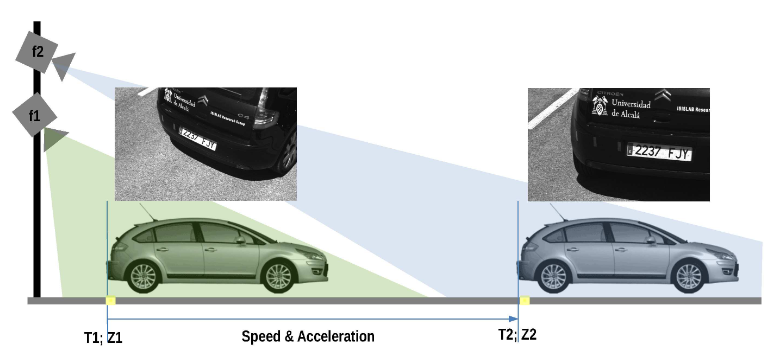
\includegraphics[width=0.75\textwidth]{Two_camera_measurement_overall_view}
\end{linfigure}

As seen in figure \ref{fig:two_camera_measurement_overview} two cameras are used to record a fixed point on the road. These cameras are setup using a
fixed pole in the road. However, this setup can also be achieved using smaller constructions allowing for a clearer view of a licence plate. Using 
this setup allows for use of vision-type programming and a more linear way of licence plate recognition. Experiments have also shown that using the 
setup shown in figure \ref{fig:two_camera_measurement_overview} has a base a maximum speed error of less then 3kmh, meaning it is conform the given
requirements by the client. 

\section{VASCAR speed measuring method}
A VASCAR is a device/technique containing a stopwatch and a processor. The VASCAR starts recording time when a vehicle passes a fixed/generated spot 
on the road, after the vehicle has passed another predetermined fixed/generated spot the recording will stop. The vehicles average speed is then calculated 
by distance between points and the time taken for the vehicle to pass over them. 

Due to radar and LIDAR techniques being illegal and not being allowed by the client, the VASCAR method is a viable option due to it not relying on 
these two methods.

The camera does not have to be in line with the road, due to it being focused on a singular/dual point on the road. And it uses the following formula:
\begin{equation}
    speed = distance \div time
\end{equation}


If the formula 5.1 does not work conform the measurement requirements, the following formulas can be used to calculate the average speed of an object:
\begin{equation}
    Meters Per Pixel = mmp = Distance Constant \div Frame Width
\end{equation}
\begin{equation}
    Distance In Pixels = p_{ab} = | col_A - col_B |
\end{equation}
\begin{equation}
    Distance In Meters Zone_{ab} = d_{ab} = p_{ab} \times mmp
\end{equation}
\begin{equation}
    Average Speed = \Delta t_{ab} \div d_{ab}
\end{equation}

\subsection{Object tracking}
The cameras FOV can be used as beginning and end points for speed measurements, meaning you start measuring object as soon as they are visible on the 
camera. This also allows the device to measure the speed of objects from left-to-right and right-to-left. An object detector and centroid tracker are 
a possibility for this approach, using OpenCV. See LINK TO LICENCE RECOGNITION for a possible AI or algorithm the realize this.

A centroid tracker can be used to track the center of an object, and to use this to measure time required to pass through the cameras view. An example 
of centroid tracking can be seen in figure 1.

\begin{figure}[h]
    \caption{Example of how centroid tracking works}
    \centering
    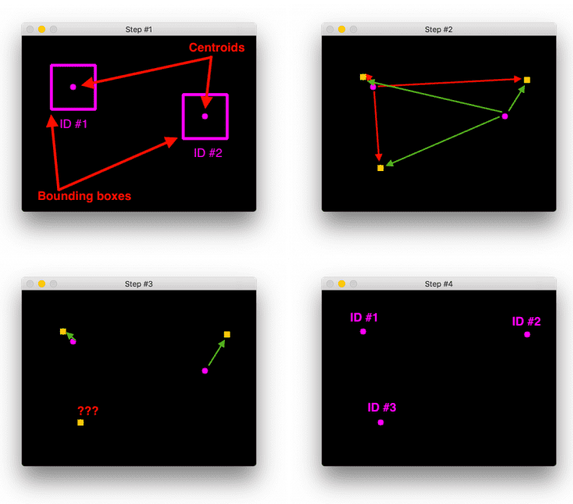
\includegraphics[width=0.75\textwidth]{Centroid_tracking_example}
    \label{fig:centroid_example}
\end{figure}

\begin{lintable}{tbl:steps_in_centroid_example}{Steps displayed in figure \ref{fig:centroid_example}}
    \begin{lintabular}{l|l}
        \lintablehead{Step & Step description}
        \lintablerow{1 & Accept bounding box coordinated and calculate the center of objects. (First frame with existing object)}
        \lintablerow{2 & Calculate distance between new bounding boxes and existing objects. (Frame where a new object is detected)}
        \lintablerow{3 & Update x,y-coordinates of existing objects. (One unknown due to new object)}
        \lintablerow{4 & Register new objects and deregister old objects.}
    \end{lintabular}
\end{lintable}



\linappendix
\chapter{\REVIEW{Development Board Comparison}}
\label{app:board-comparison}

\section{Hardware}

\cref{tbl:board-comparison} shows the differences in hardware between the Jetsen Nano Developer Kit and the Raspberry Pi 4.
These board have many similarities in hardware. They are both equipped with an ARM CPU (Central Processing Unit) and 4 GB of LPDDR4 (Low-Power Double Data Rate) memory.
The biggest difference between these board is that the RPI 4 has an Broadcom VideoCore VI, and the Jetson Nano has a much more powerful 128-core Maxwell GPU (Graphics Processing Unit).

\begin{lintable}{tbl:board-comparison}{Board Hardware Comparison}
    \begin{lintabular}{l|l|l}
        \lintablehead{       & Jetson Nano Developer Kit    & Raspberry Pi 4}
        \lintablerow{CPU     & Quad-core ARM A57 @ 1.43 GHz & Quad-core ARM Cortex-A72 @ 1.5 GHz}
        \lintablerow{Memory  & 4 GB 64-bit LPDDR4 25.6 GB/s & 4 GB LPDDR4-3200}
        \lintablerow{GPU     & 128-core Maxwell             & Broadcom VideoCore VI}
        \lintablerow{Camera  & 2x MIPI CSI-2 DPHY lanes     & 2-lane MIPI CSI camera port}
    \end{lintabular}
\end{lintable}

The data in this table is retrieved from \cite{nvidia:jetson-nano-datasheet} and \cite{rpiltd:raspberry-pi-datasheet}.

\cref{tbl:gpu-comparison} displays the difference between the GPUs.
You can see that the Maxwell GPU has around 8 times better performance then the VideoCore VI.

\begin{lintable}{tbl:gpu-comparison}{GPU Comparison}
    \begin{lintabular}{l|l|l}
        \lintablehead{                   & 128-core Maxwell & Broadcom VideoCore VI}
        \lintablerow{Performance (GLOPS) & 512              & 64}
        \lintablerow{Clock speed (MHZ)   & 921              & 500}
    \end{lintabular}
\end{lintable}

The data in this table is retrieved from \cite{nvidia:jetson-nano-datasheet} and \cite{gdgtvs:videocore-vi-benchmark}.

\section{Interfaces}
\label{sec:board-comparison-interfaces}

As shown in \cref{tbl:board-comparison}, both devices support MIPI CSI-2 (Camera Serial Interface).
Both device also have a Gigabit Ethernet port. However, the RPI 4 also has 802.11 b/g/n/ac Wireless LAN and the Jetson Nano does not.


\end{document}
